\documentclass[18pt,letterpaper]{article}
\usepackage{cvpr}
\usepackage{times}
\usepackage{epsfig}
\usepackage{graphicx}
\usepackage{amsmath}
\usepackage{amssymb}

% Include other packages here, before hyperref.

% If you comment hyperref and then uncomment it, you should delete
% egpaper.aux before re-running latex.  (Or just hit 'q' on the first latex
% run, let it finish, and you should be clear).
%\usepackage[pagebackref=true,breaklinks=true,letterpaper=true,colorlinks,bookmarks=false]{hyperref}

\cvprfinalcopy % *** Uncomment this line for the final submission
\def\httilde{\mbox{\tt\raisebox{-.45ex}{\symbol{126}}}}

% Pages are numbered in submission mode, and unnumbered in camera-ready
\ifcvprfinal\pagestyle{empty}\fi


\begin{document}

\begin{abstract}
In this report we train and test a set of classifiers like logistic regression and neural net with backpropagation for object recognition.After exploring these classifiers we look at deep learning techniques like Sparse Autoencoders which is a unsupervised method to learn good representation of features from images.We use the features extracted from sparse autoencoder to build a deep network for Object Recognition.
\end{abstract}
\section{Introduction}
An object recognition system finds object in the real world from an images of the world,using object classes which are known a priori.In this report we will discuss the different types of classification algorithms that can be used for building a model for object recognition and analyze their classification accuracy on the test set.The task is to predict the labels of images from the given categories of digits which ranges from 0-9.We first train the dataset with differnt classifiers like Neural Networks with backpropagation and Logistic Regression on the raw image pixels.We than explore unsupervised methods like Sparse Autoencoders which can learn good representation of features from the image pixels.We finally build a Deep Network using approaches we learned above for Object Recognition.
\section{The Dataset}
The data for the task is taken from the MNIST (Modified National Institute of Standards and Technology) dataset.The MNIST database contains 42,000 digits ranging from 0 to 9 for training the digit recognition system, and another 28,000 digits as test data. Each digit is normalized and centered in a gray-level image with size 28 28, or with 784 pixel in total as the features. 
\begin{figure}[ht!]
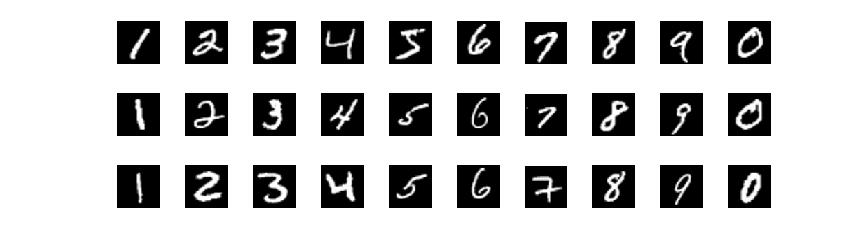
\includegraphics[width=8cm]{pic.jpg}
\end{figure}
\section{Training}
We describe here all the training approaches we have taken to train the classifier for multiclass object detection.We also give the classification accuracy of our training algorithms on the test test.
\subsection{Logistic Regression}
We will be using multiple one-vs-all logistic regression model to build a
multi-class classifier. Since there are 5
classes, we will need to train 5 separate logistic regression classifiers.
The cost function for logistic regression is:$$J=\frac{1}{m}\sum\limits_{i=1}^m[-y^{(i)}\log(h\theta(x^{(i)}))-(1-y^{(i)})\log(1-h\theta(x^{(i)}))]$$
Here,
$$ h\theta(x)=\frac{1}{1 + e^{-x}} $$
We let $ x_0=1 $, so that $x \in \Re^{n+1}$
and $ \theta \in \Re^{n+1} $, and $ \theta_0 $ is the intercept term.  We have a training set
$ \{(x^{(1)}, y^{(1)}), \ldots, (x^{(m)}, y^{(m)})\} $ of $m$ examples, and the batch gradient
ascent update rule is $ \theta := \theta + \alpha \nabla_\theta \ell(\theta) $, where $ \ell(\theta) $
is the log likelihood and $ \nabla_\theta \ell(\theta)$
We thus compute the gradient:
$$
\nabla_\theta \ell(\theta) = \sum_{i=1}^m \left(y^{(i)} - h_\theta(x^{(i)}) \right) x^{(i)}_j.
$$
We have a training set of 500 examples.There are 240 feature vectors for each training set.Each feature represents a keypoint extracted from the image using standard algorithms.With these feature we train our clasifier using one vs all approach of Logistic Regression.After training we obtain a set of parameters which we can be used to predict the labels of the test set and can determine its accuracy.
\subsection{Neural Nets with BackPropagation}
We use now Neural Networks which give a way of defining a complex,
non-linear form of hypotheses $h_{W,b}(x)$,with parameters $W,b$ that we can
fit to our data.To describe neural networks, we will begin by describing the simplest possible
neural network, one which comprises a single "neuron."
The "neuron" is a computational unit that takes as input $x_1, x_2, x_3$ (and a +1 intercept term), and
outputs $\textstyle h_{W,b}(x) = f(W^Tx) = f(\sum_{i=1}^3 W_{i}x_i +b)$, where $f : \Re \mapsto \Re$ is
called the 'activation function'.
$$ f(z) = \frac{1}{1+\exp(-z)} $$
A neural network is put together by hooking together many of our simple
"neurons," so that the output of a neuron can be the input of another.  For
example, here is a small neural network:
\begin{figure}[ht!]
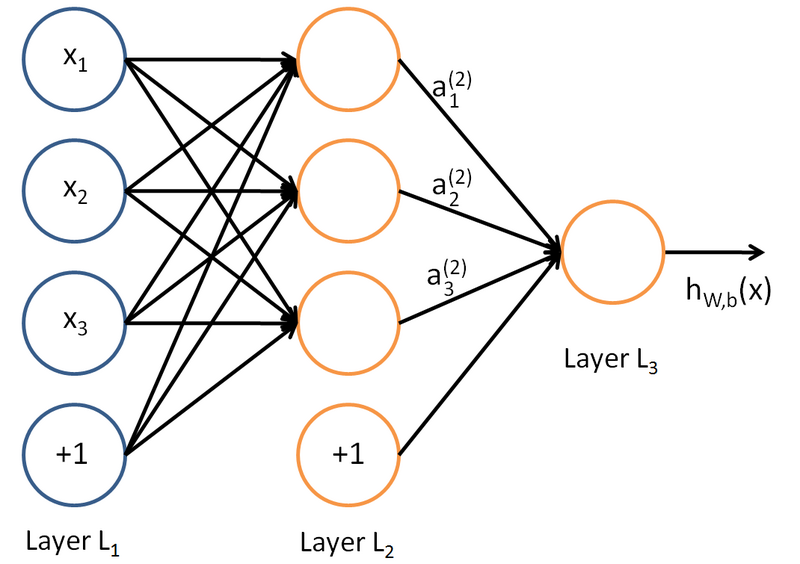
\includegraphics[width=8cm]{1.png}
\end{figure}
In this figure, we have used circles to also denote the inputs to the network.  The circles
labeled "+1" are called '''bias units''', and correspond to the intercept term.
The leftmost layer of the network is called the '''input layer''', and the
rightmost layer the '''output layer'''.The middle layer of nodes is called the '''hidden layer''', because its
values are not observed in the training set.  We also say that this example
neural network has 3 '''input units''' (not counting the bias unit), 3 
'''hidden units''', and 1 '''output unit'''.
We will let $n_l$ denote the number of layers in our network.
The neural network has parameters $(W,b) = (W^{(1)}, b^{(1)}, W^{(2)}, b^{(2)})$, where
$W^{(l)}_{ij}$ denote the parameter (or weight) associated with the connection
between unit $j$ in layer $l$, and unit $i$ in layer $l+1$.Also,$b^{(l)}_i$ is the bias associated with unit $i$ in layer $l+1$
Given a fixed setting of the parameters $W,b$,our neural network defines a hypothesis $h_{W,b}(x)$ that outputs a real number.
$$a_1^{(2)} = f(W_{11}^{(1)}x_1 + W_{12}^{(1)} x_2 + W_{13}^{(1)} x_3 + b_1^{(1)})$$
$$a_2^{(2)} = f(W_{21}^{(1)}x_1 + W_{22}^{(1)} x_2 + W_{23}^{(1)} x_3 + b_2^{(1)})$$
$$ a_3^{(2)} = f(W_{31}^{(1)}x_1 + W_{32}^{(1)} x_2 + W_{33}^{(1)} x_3 + b_3^{(1)})$$
$$h_{W,b}(x) = a_1^{(3)} =  f(W_{11}^{(2)}a_1^{(2)} + W_{12}^{(2)} a_2^{(2)} + W_{13}^{(2)} a_3^{(2)} + b_1^{(2)})$$
We call this step forward propagation.Neural networks can also have multiple output units.
Suppose we have a fixed training set $\{ (x^{(1)}, y^{(1)}), \ldots, (x^{(m)}, y^{(m)}) \}$ of $m$ training examples. We can train our neural network using batch gradient descent. In detail, for a single training example $(x,y)$, we define the cost function with respect to that single example to be:
$$ J(W,b; x,y) = \frac{1}{2} \left\| h_{W,b}(x) - y \right\|^2$$
This is a (one-half) squared-error cost function.The goal is to minimize $J(W,b)$ as a function of $W$ and $b$.We use backpropagation algorithm to minimize this cost function and get optimal set of weights to make predictions.We use the same training set to train the classifier to make predictions and record its classification accuracy on the test set.
\subsection{Sparse Autoencoders}
Suppose we have only a set of unlabeled training examples $\textstyle \{x^{(1)}, x^{(2)}, x^{(3)}, \ldots\}$,
where $\textstyle x^{(i)} \in \Re^{n}$.An autoencoder neural network is an unsupervised learning algorithm that applies backpropagation,setting the target values to be equal to the inputs.
\begin{figure}[ht!]
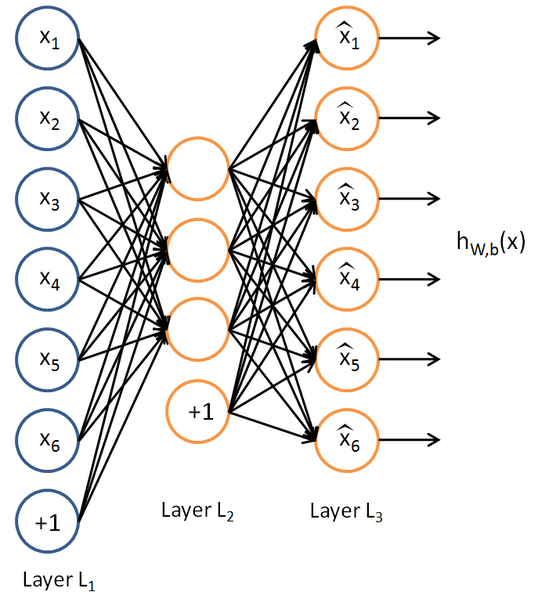
\includegraphics[width=8cm]{2.png}
\end{figure}
The autoencoder tries to learn a function $\textstyle h_{W,b}(x) \approx x $.In other
words, it is trying to learn an approximation to the identity function, so as
to output $\textstyle \hat{x}$ that is similar to $\textstyle x$.The identity function seems a
particularly trivial function to be trying to learn but by placing constraints
on the network, such as by limiting the number of hidden units, we can discover
interesting structure about the data.
Informally, we will think of a neuron as being active if its output value is close to 1, or as being inactive if its output value is
close to 0.We would like to constrain the neurons to be inactive most of the
time. 
$\textstyle a^{(2)}_j$ denotes the activation of hidden unit $\textstyle j$ in the
autoencoder.However,this notation doesn't make explicit what was the input $ x $
that led to that activation.Thus, we will write $\textstyle a^{(2)}_j(x)$ to denote the activation
of this hidden unit when the network is given a specific input $\textstyle x$.  Further, let
$$\hat\rho_j = \frac{1}{m} \sum_{i=1}^m \left[ a^{(2)}_j(x^{(i)}) \right]
$$ be the average activation of hidden unit $\textstyle j$.
We would like to (approximately) enforce the constraint
$ \hat\rho_j = \rho,$
where $\textstyle \rho$ is a sparsity parameter, typically a small value close to zero
.In other words, we would like the average activation
of each hidden neuron $\textstyle j$ to be close to 0.05 (say).To satisfy this
constraint, the hidden unit's activations must mostly be near 0.
To achieve this, we will add an extra penalty term to our optimization objective that
penalizes $\textstyle \hat\rho_j$ deviating significantly from $\textstyle \rho$.We will choose the following cost function to train sparse autoencoder and backpropagation algorithm to obtain optimal weights.
$$
\sum_{j=1}^{s_2} \rho \log \frac{\rho}{\hat\rho_j} + (1-\rho) \log \frac{1-\rho}{1-\hat\rho_j}.
$$

\subsection{Deep Networks for Classification}
Using all the techniques we learnt above we now build a deep network for object classification.We will use standard MNSIT handwritten digits for our task.First we will take 10,000 examples from the data set whose label is unknown to us.We will feed this data to the sparse autoencoder.The sparse autoencoder try to learn weights to represent the image in a more compressed form.If we visualize these learned weights it looks like detecting edges at different positions in the image.

\begin{figure}[ht!]
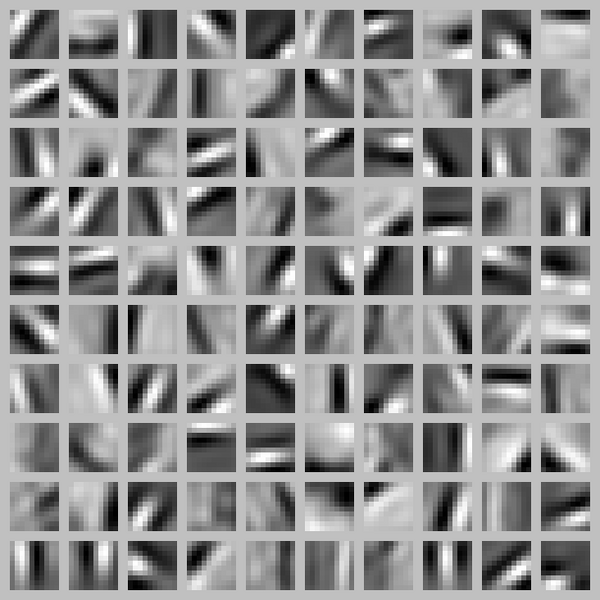
\includegraphics[width=8cm]{6.png}
\end{figure}

Each square in the figure above shows the input image that maximally actives one of the hidden units. We see that the different hidden units have learned to detect edges at different positions and orientations in the image.We save this learned weights to get good features from images whose labels are already known to us.
We have a labeled training set that we can replace the original features with features computed by the sparse autoencoder.We do this by multiplying the weights we get from sparse autoencoder with the training set.This gives us a new training set.Finally, we train a logistic classifier to map from the features $a^{(i)}$ we laerned above to the classification label $y^{(i)}$.The overall architecture looks like below:  
\begin{figure}[ht!]
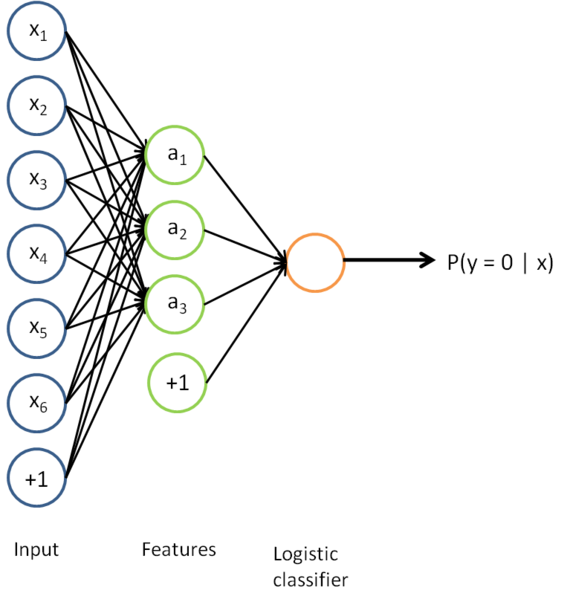
\includegraphics[width=8cm]{7.png}
\end{figure}

Here we constructed a 3-layer neural network comprising an input, hidden and output layer. While fairly effective for MNIST,this 3-layer model is a fairly shallow network which means that the features are computed using only one layer of computation.
We build a deep neural networks in which we have multiple hidden layers.This will allow us to compute much more complex features of the input because each hidden layer computes a non-linear transformation of the previous layer,so a deep network can have significantly greater representational power than a shallow one.One method that has been used is the greedy layer-wise training method.The idea is to train the layers of the network one at a time, so that we first train a network with 1 hidden layer, and only after that is done, train a network with 2 hidden layers, and so on. At each step, we take the old network with $k\mathbin{-}1$ hidden layers, and add an additional k-th hidden layer.So here we use a 3 layer deep network.The weights that we obtain from running sparse autoencoder are again fed into a new sparse autoencoder which can learn a more compressed represntation of the learned weights.The weights from training the layers individually are then used to initialize the weights in the final deep network and only then is the entire architecture is trained together to optimize the labeled training set error.

We observe the overall performance improves significantly using deep networks.


\subsection{Pre-Processing of Data}
Data preprocessing plays a very important in many deep learning algorithms. In practice,we have seen our performance improved between 2-7 perecent after our data has been pre-processed before using it to train a classifier.We used simple rescaling,in which our goal was to rescale the data along each data dimension (possibly independently) so that the final data vectors lie in the range $[0, 1]$ or  $[-1, 1]$.We also tried feature standardization which refers to setting each dimension of the data to have zero-mean and unit-variance. This is the most common method for normalization. We achieved this by first computing the mean of each dimension (across the dataset) and subtracts this from each dimension. Next,each dimension is divided by its standard deviation.Out of the two approaches we found z-score to perform better on RGB images.
\subsection{PCA/ZCA}
PCA(Principal Component Analysis) will allow us to approximate the input with a much lower dimensional one, while incurring very little error.
Whitening is a preprocessing step which removes redundancy in the input, by causing adjacent pixels to become less correlated.
Since grey-scale images have the stationarity property, we usually first remove the mean-component from each data example separately.After this step, PCA/ZCA whitening is often employed with a value of epsilon set large enough to low-pass filter the data.

\subsection{Results}

\begin{tabular}{|c|c|}
\hline 
Training Method & Classification Accuracy \\ 
\hline 
Logistic Regression & 78\% \\ 
\hline 
Neural Net & 88\% \\ 
\hline 
Deep Learning & 92\% \\ 
\hline 
\end{tabular} 
The code\footnote{https://github.com/manishrocksag/ObjectRecognition}
for the all of the implementation can be found in the online repository. 

\begin{thebibliography}{9}

\bibitem{1}
Rajat Raina,Alexis Battle,Honglak Lee,Benjamin Packer,Andrew Y. Ng
  \emph{Self-taught Learning: Transfer Learning from Unlabeled Data}. Computer Science Department, Stanford University, CA 94305 USA

\bibitem{2}
Rajat Raina,Anand Madhavan,Andrew Y. Ng 
  \emph{Large-scale Deep Unsupervised Learning using Graphics Processors
}.
Computer Science Department, Stanford University, CA 94305 USA
  
\bibitem{3}
  Yoshua Bengio
  \emph{Learning Deep Architectures for AI
}.
Dept. IRO, Universit´e de Montr´eal
C.P. 6128, Montreal, Qc, H3C 3J7, Canada

\bibitem{4}
  Memisevic,Hinton G. E.
  \emph{Unsupervised learning of image transformations.}.
Computer Vision and Pattern Recognition (CVPR-07)


\end{thebibliography}

\end{document}
